\documentclass[]{article}
\usepackage[top=1.2cm,bottom=1.5cm,left=1.2cm, right=1.2cm,bindingoffset=0.6cm]{geometry}
\usepackage{graphicx}
\usepackage{lscape}

\usepackage{listings}
\usepackage{color}
\definecolor{dkgreen}{rgb}{0,0.6,0}
\definecolor{gray}{rgb}{0.5,0.5,0.5}
\definecolor{mauve}{rgb}{0.58,0,0.82}

\lstset{frame=tb,
	language=Python,
	aboveskip=3mm,
	belowskip=3mm,
	showstringspaces=false,
	columns=flexible,
	basicstyle={\small\ttfamily},
	numbers=none,
	numberstyle=\tiny\color{gray},
	keywordstyle=\color{blue},
	commentstyle=\color{dkgreen},
	stringstyle=\color{mauve},
	breaklines=true,
	breakatwhitespace=true,
	tabsize=3
}

% Title Page
\title{Autómatas en dos dimensiones tipo Life \\\hfill\break Sistemas Complejos}
\author{Prof: Genaro Juárez Martínez \\ \\ Luis Eduardo Valle Martínez}
\date{24 de Abril del 2022}


\begin{document}
\maketitle

\section{Introducción}
% https://revistacienciasunam.com/es/172-revistas/revista-ciencias-24/1572-una-introducci%C3%B3n-a-aut%C3%B3matas-celulares.html
% https://kryptonsolid.com/que-es-un-automata-celular-ca-y-para-que-se-utiliza/
% https://isolution.pro/es/q/cs13075500/como-funcionan-las-reglas-de-los-automatas-celulares-2d
% https://delta.cs.cinvestav.mx/~mcintosh/comun/tesismaestria/genaro/node5.html
% 
	Este reporte técnico tiene como objetivo explicar y documentar la solución propuesta mediante el diseño y desarrollo de un simulador de espacios de evolución de Autómatas Celulares en 2 dimensiones mediante reglas de evolución definidas, siendo el referente base el trabajo desarrollado por el matemático británico John Horton Conway, el Juego de la Vida de Conway.
	
	Este juego se trata de un juego tipo jugador zero, donde la evolución del sistema está determinado por un estado inicial y no requiriendo otra entrada para observar su evolución.
	
	El universo del Juego de la Vida es teóricamente un espacio infinito, una rejilla ortogonal bidimensional de células cuadradas, de las cuales pueden tomar 2 únicos valores(Viva o Muerta), correspondiento al alfabeto $\Sigma = {0,1}$. Cada una de las células interactua con sus 8 vecinos que la rodea, llamada vecindad de Moore(ventana del espacio de evolución de tamaño 3x3 donde la célula ancla ubicada en el centro de la ventana interactua con las células que la rodean para definir el estado siguiente en una nueva generación).
	
	Por términos prácticos, el universo de una simulación del juego de la vida no puede ser inifinito, por lo que se suele indicar el tamaño de espacio de evolución antes de iniciar la ejecución del programa con un valor asignado a una constante de configuración.
	
	Las evoluciones del universo en la simulación dependerá en cada célula por su vecindad de Moore, rigiéndose por una regla que indica según el número de vecinos adyacentes vivos el nuevo estado que toma la célula. Para la regla del Juego de la Vida las condiciones son las siguientes:
	\begin{enumerate}
		\item Cualquier célula viva con 2 o 3 vecinos vivos sobrevive.
		\item Cualquier célula muerta con exactamente 3 vecinos se converte en una célula viva(Nacimiento).
		\item Cualquier célula con más de 3 vecinos vivos muere por sobrepoblación
		\item Cualquier célula con menos de 2 vecinos vivos mere por subpoblación
	\end{enumerate}
	Por naturaleza esta implementación de reglas se realiza simultaneamente en cada célula obteníendose los nuevos valores de las células en el mismo instante. Cada generación es una función pura de las precedentes. Esta regla es implementada repetidamente para la creación de futuras generaciones.
	
	El desarrollo se realizó utilizando el lenguaje de programación Python con el uso de la biblioteca PyGame como principal bilioteca gráfica, Numpy para el manejo eficiente de estructuras como \textit{arrays} para los espacios de evolución, Matplotlib para la graficación de los análisis estadísticos y finalmente Numba como traductor de funciones Python a funciones paralelizables con aceleración por hardware gracias al controlador CUDA de NVIDIA para sus GPUs.
	
	La simulación ofrece su funcionalidad mediante el control enteramente desde la interfaz, la cual se diseño considerando una fácil e intuitiva interacción para los usuarios, el mayor aprovechamiento del espacio y estructura de los componentes que la compone y finalmente un diseño agradable y consistente que pueda ser común con otras interfaces populares acelerando la adaptación de un nuevo usuario con la aplicación.
	
	En secciones posteriores se realizará el desglose del programa en sus dependencias requeridas para se ejecución, requsitos funcionales del programa, interfaz y su conformación, elementos gráficos, su funcionalidad y operación, la implementación de optimización mediante aceleración por hardware, características del espacio de evolución y exposición de todas las funcionalidades de este, ejemplos de la simulación corriendo a diferentes tamaño de evolución, graficación de las medidas de análisis estadístico por generaciones, y finalmente el código fuente del programa completo.
	
\newpage

\section{Programa}
	\subsection{Dependencias}
		
		A continuación se listan las dependencias de bibliotecas, programas y hardware requeridos para la ejecución del programa.
		
		El programa fue desarrollado utilizando el lenguaje de programación Python por lo que se requiere minimamente la instalación de Python en culquiera de sus versiones 3, siendo desarrollado en la versión 3.9.7.
		
		Las bibliotecas listadas a continuación pueden ser instaladas mediante programas como \textit{pip}, o directamente en un ambiente virtual como \textit{pipenv} o \textit{anaconda}:
		\begin{itemize}
			\item PyGame 2.1.2
			\item Numpy 1.21.5
			\item Matplotlib 3.5.1
			\item Numba 0.55.1
		\end{itemize}
	
		\hfill \break
		\textbf{PyGame} es una biblioteca utilizada para el desarrollo de sencillos juegos 2D en python, incluyendo algunas herramientas gráficas para la impresión en pantalla de diferentes forma geométricas, imágenes y Sprites. Incluye métodos usados para la detección de colisiones entre objetos, impresión de áreas en pantalla y otros de configuración como el número de veces de refresco de pantalla en cuadros por segundo FPS(\textit{Frames Per Second}).
		Incluye así también métodos para la fácil implementación de sonido y archivos de audio, sin embargo este tipo de funciones no se utilizan en el desarrollo de este programa.
		
		\hfill \break
		
		\textbf{Numpy} es un biblioteca para el manejo de vectores y matrices, incluyendo un amplio conjunto de recursos en funciones matemáticas en el dominio del algebra lineal, transformada de fourier y matrices.
		Principalmente el uso de esta biblioteca en el programa se encuentra en el uso de \textit{arrays} como estructuras para el manejo de espacios y otros recursos auxiliares que permiten de forma sencilla y eficiente las operaciones durante la evolución del espacio bidimensional de los autómatas.
		Importante señalar que los \textit{arrays} y algunas operaciones de \textit{numpy}, son las estructuras básicas y funciones matemáticas válidas en \textit{Kernels} y funciones numba utilizadas para el procesamiento con CUDA.
		
		\hfill \break
		
		\textbf{Matplotlib} es una biblioteca utilizada para la creación de visualizaciones estáticas, animadas e interactivas en Python. Esta biblioteca provee funciones que permiten la graficación de las diferentes medidas de complejidad.
		
		\hfill \break
		
		\textbf{Numba} es una biblioteca de Python que traduce funciones a código máquina optimizando el tiempo de corrida utilizando la biblioteca de compilación estándar en la industria LLVM. Algoritmos numéricos compilados por Numba en Python pueden alcanzar velocidades de C o Fortran, a través de la paralelización de algoritmos ofreciendo un rango de opciones utilizando CPUs y GPUs.
		En el programa se utiliza una alternativa de aceleración de hardware al tener soporte para CUDA de Nvidia y ROCm de AMD para sus tarjetas gráficas. Mediante la creación de \textit{Kernels}(Función ejecutada en un número de bloques con N números de hilos de ejecución para cada bloque), esto resulta conveniente pues el tiempo de procesamiento de los \textit{array} se mantiene relativamente constante pues se ocupan NxM hilos siendo NxM el tamaño del \textit{array}.
		
		\hfill \break
		
		La totalidad del proceso de desarrollo y pruebas del funcionamiento de la simulación se realizó utilizando un SO llamado Pop!\_OS en su versión 21.10, sistema basado en UNIX Linux derivado de la popular distribución Debian.
		Se utilizó un ambiente virtual para la ejecución de la simulación, con la instalación de dependencias únicamente en este ambiente y no todo el SO con la herramienta \textit{pipenv} de Python.
		
		\hfill \break
		
		La ejecución del programa en otro sistema operativo diferente a una distribución Linux no debería ser impedida si se cuenta con la instalación de todas las dependencias, ya sea en un ambiente virtual o directamente en el ambiente de trabajo del usuario. El único inconveniente que pudiera surgir aún con las depedencias instaladas es el uso de la aceleración por hardware, si el equipo que se utiliza no cuenta con una tarjeta gráfica dedicada de NVIDIA o AMD, es necesario modificar la constante de configuración \textbf{GPU\_ENHANCEMENT} a \textit{False} en la línea 28 del archivo \textit{main.py}.
	
		\subsubsection{Hardware}
			A raíz de la optimización del programa para su ejecución con la ayuda de aceleración por GPU se requiere contar evidentemente con una GPU, sin importar sea de NVIDA o AMD.
			
			Requiriendo si por su parte, la instalación de los controladores CUDA para NVIDIA y ROCm para AMD en el sistema.
			
			La aceleración por GPU refiere a la paralelización de los algoritmos realizados principalmente sobre estructuras tipo \textit{arrays}, dando la posibilidad de ejecutar una función para cada elemento del array en un núcleo propio y lo que permite se acelere mucho el tiempo de corrida de un algoritmo que en un CPU correría secuencialmente mientras que con la GPU tomaría un tiempo comparable a la ejecución de la función para 1 de los elementos del \textit{array} con la típica ejecución mediante CPU.
			
	\newpage
	\subsection{Requerimientos}
		El programa consiste en un simulador gráfico de un espacio de evoución para una cierta configuración de Autómatas Celulares en 2 dimensiones, basado en el "Juego de la vida" de Conwell. Precisamente la evolución se realiza siguiendo una tupla de números que corresponde a una regla, dependiendo del valor de estos 4 números y el número de vecinos en una vecindad de Moore, en la siguiente evolución la célula ancla puede Vivir, Morir o Nacer, dependiendo el estado nuevo también del estado actual de la célula(Viva o Muerta).
		
		\hfill \break
		Para facilitar el uso del simulador y precisamente poder observar la evolución de una manera intuitiva en forma de animación, el programa requirió de una implementación gráfica, aprovechandose esta cualidad para incluir botones o diferentes componenetes que permitan al usuario configurar los parámetros y condiciones en el que tendrá lugar el proceso de evolución para la configuración del espacio.
		
		\hfill \break
		A continuación se numeran los requerimientos funcionales con las que el programa debe cumplir:
		
		\begin{enumerate}
			\item Evaluación de espacios de 300x300, 500x500 y máximo de 1000x1000 células
			\item Animación en 2 dimensiones
			\item Poder cambiar los colores de los estados
			\item Inicialización del espacio de evoluciones con diferentes densidades
			\item Edición del espacio de evoluciones para dibujar configuraciones particulares
			\item Salvado y levantado de archivos con configuraciones en específico
			\item Graficación de:
				\begin{itemize}
					\item Densidad(número células vivas) por generación
					\item Logaritmo base 10 de la Densidad por generación
					\item Entropía
				\end{itemize}
			\item Especificación de las reglas de evolución en notación: $R(S_{min},S_{max},B_{min},B_{max})$
		\end{enumerate}
	
	\newpage
	\subsection{Interfaz}
		Como se mencionó en la sección de \textbf{Dependencias}, la principal biblioteca para los elementos gráficos del simulador fue \textit{PyGame}.
		
		Aún con las herramientas y funciones que provee esta biblioteca, se considera una biblioteca de nivel bajo, facilitando tan solo herramientas básicas para la construcción completa de un videojuego, lo que ya en un principio presenta un conjunto de retos que se exponen posteriormente, así como la solución con la que se abordaron estas limitaciones.
		
		Importante es tomar en cuenta que como una biblioteca enfocada a videojuegos, no se proveé prácticamente facilidad alguna para la creación de interfaces gráficas con los típicos elementos gráficos como botones, sliders, etc. Se resalta esto pues existen bibliotecas sencillas en Python como \textit{TKinter} o incluso \textit{Frameworks} ya más complejos como \textit{PySide 6}, que proveen herramientas avanzadas para la creación sencilla de interfaces gráficas, con la posibilidad de implementar diseños modernos con funcionalidades intuitivas sin demasiada dificultad. El caso de \textit{PyGame} es lo contrario, todos los elementos gráficos e incluso de estructura, fueron implementados desde 0 construyendose con formas básicas como rectángulos, círculos, iconos e inclusive el posicionamiento de los elementos se realiza a nivel coordenadas de pixel dentro la ventana.
		
		Ya creados estos elementos básicos gráficos para conformar una interfaz, en conjunto de los elementos de organización y posición, se muestra en la figura \ref{Interfaz} la interfaz final del simulador.
		
		\begin{figure}[!h]
			\centering
			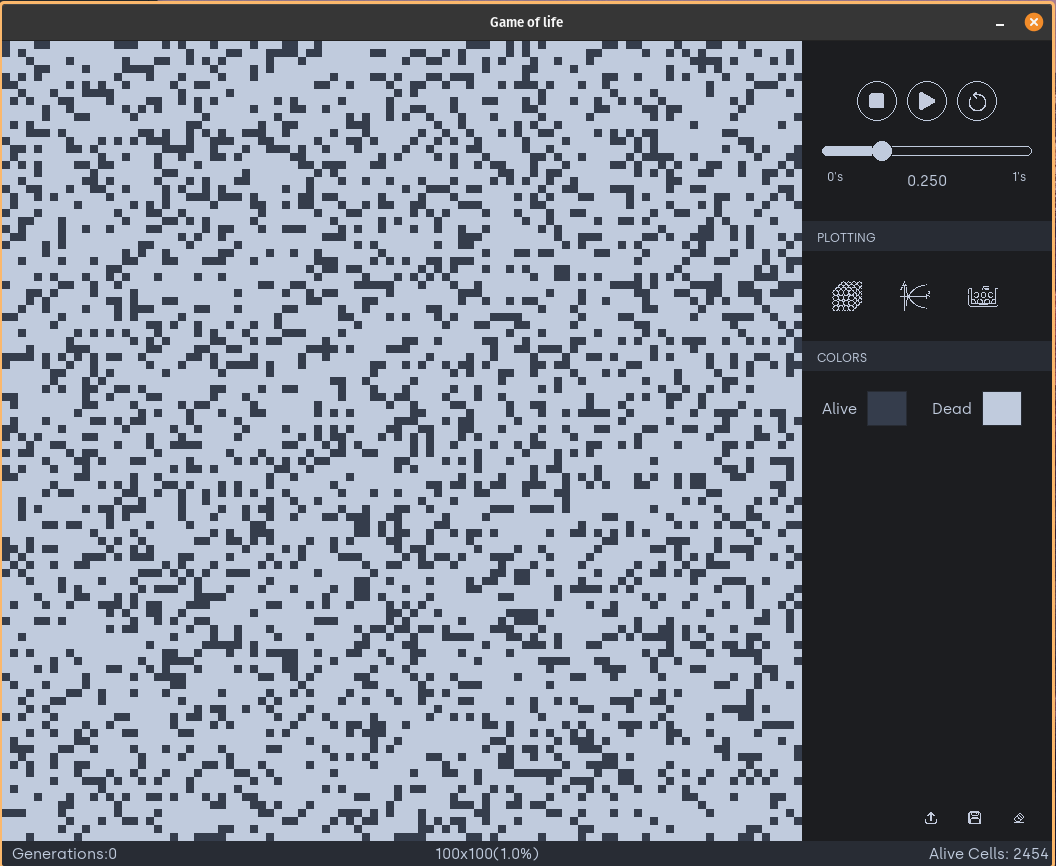
\includegraphics[width=15cm]{Imagenes/Interfaz.png}
			\label{Interfaz}
			\caption{Captura de pantalla de la interfaz gráfica del simulador al ejecutarse}
		\end{figure}
	
		\subsubsection{Componentes Gráficos}
			Todos los componenetes gráficos que se describen pertenecen al módulo de la aplicación nombrado \textit{GraphicalComponents} y que puede verse su implementación Python en la sección de \textbf{Código Fuente}.
			
			\paragraph{Botón}
				Los botones son componentes gráficos básicos en cualquier GUI, y no es excepción en el programa de simulación pues se utilizan un total de 9 botones y que permiten desempeñar diferentes acciones.
				
				\hfill \break
				La primer triada de botones son los utilizados para Pausar, Correr y Cargar una nueva configuración de la simulación. Ubicados en la parte superior derecha en la sección lateral, son probablemente los botones más importantes pues ejecutan las funciones básicas de evolución en la simulación.
				
				\begin{figure}[!h]
					\centering
					
\includegraphics[width=5cm]{Imagenes/botones_correr.png}
					\caption{Botones que dictan el flujo de las evoluciones del espacio 2D}
					\label{Evolution_buttons}
				\end{figure}
				
				\hfill \break
				Siguiendo en importancia ubicados en la parte inferior de la sección lateral se ubican los 3 botones de acciones relacionadas al espacio gráfico de evolución. El primero de ellos representado por un ícono de una flecha es el botón \textit{Charge} y permite cargar una configuración en un archivo CSV. Le sigue el botón con ícono de disquet \textit{Load}, que permite guardar la actual configuración del espacio de evolución. Finalmente se tiene un ícono de goma de borrar \textit{Clear}, que limpia el espacio de evolución colocando el espacio con todas las células muertas.
				
				\begin{figure}[!h]
					\centering
					
\includegraphics[width=5cm]{Imagenes/botones_inferiores.png}
					\caption{Botones inferiores para la configuración del estado de evolución}
					\label{Space_configuration_buttons}
				\end{figure}
				
				\hfill \break
				Finalmente ubicadas en la sección de \textit{Plotting}, se tienen 3 botones que se encargan de la graficación.
				El primero de ellos con un ícono de cubo corresponde a la gráfica de Densidad para las generaciones corridas. Le sigue un botón con ícono de una gráfica logarítmica, y que precisamente grafica el logaritmo de las densidades. Finalmente se tiene el ícono con unas partículas de un gas para la graficación de la Entropía.
				
				\begin{figure}[!h]
					\centering
					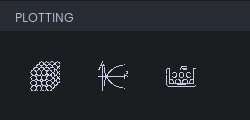
\includegraphics[width=5cm]{Imagenes/botones_plots.png}
					\caption{Botones con íconos para la graficación de la complejidad de los estados evolucionados}
					\label{Botones_graficacion}
				\end{figure}
			
			\paragraph{Texto}
				Se utilizan algunos textos para indicar el estado actual del espacio de evolución, siendo los 3 más importantes aquellos impresos en la barra inferior, y que respectivamente indican el número de generaciones que han transcurrido, el tamaño del espacio y entre paréntesis la escala de zoom(Funcionalidad no disponible con la versión de la simulación en el tiempo en el que se redacta el reporte), y finalmente el número de células en el espacio que se encuentran vivas.
				
				\begin{figure}[!h]
					\centering
					
\includegraphics[width=12cm]{Imagenes/textos_seccion_inferior.png}
					\caption{Textos ubicados en la barra inferior. Con el proposito de mostrarlos los 3 la imagen se ha recortado para ubicarlos juntos, sin embargo en la interfaz se muestran en las esquinas y el centro de la ventana en la parte inferior}
				\end{figure}
			
			\paragraph{Slider}
				Un slider es un componente gráfico algo más complejo que va a estar formado por una combinación de los 2 elementos anteriores así como un par de rectángulos y círculos que le dan forma al cuerpo de la ranura por la que el botón se desliza.
				
				La función de este slider es la elección del complemento de la densidad, y que es aplicado cuando se da al botón Reset que carga una nueva configuración de espacio de evolución con un número aleatorio de células vivas que se rigen por el complemento de la probabilidad que se escoge con el slider.
				
				\begin{figure}[!h]
					\centering
					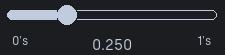
\includegraphics[width=8cm]{Imagenes/slider.png}
					\caption{Slider para elegir la probabilidad de las células muertas cuando se realiza un Reset}
					\label{Slider}
				\end{figure}
			
			\paragraph{Input}
				El input es un elemento típicamente utilizado en formularios para el ingreso de texto corto. El input cuenta con una \textit{Label} etiqueta que sirve al usuario para indicar el tipo de respuesta que se debe colocar ahí, asi como del cuerpo del input y el texto por supuesto.
				
				Un uso poco convecional pero conveniente por su previo desarrollo e implementación en el programa de ECA en 1 dimensión, un par de inputs se utilizan como una clase de botones que permiten el cambio de los colores para las células vivas o muertas.
				
				Se opto por utilizarse estos elementos por el texto de etiqueta que por defecto se coloca en el input, colocándose un texto vació e ignorando eventos de tecla que los pueda modificar, siendo únicamente el click el que desencadene la función para el cambio de color.
				
				Los colores disponibles pueden consultarse en el módulo \textit{Constants} en la sección \textbf{Código Fuente}.
				
				\begin{figure}[!h]
					\centering
					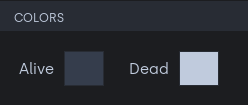
\includegraphics[width=7cm]{Imagenes/colores.png}
					\caption{Par de inputs ubicados en la sección \textit{Colors} y que permiten modificar el color actual de las células vivas y muertas}
					\label{Colores_celulas}
				\end{figure}
				
			
			\paragraph{Células Gráficas}
				Este componenete gráfico es el único que no se encuentra en el módulo \textit{GraphicalComponents} pues se encuentra declarado en el módulo \textit{Graphics}, esto se debe a que a diferencia de los elementos anteriores las células no son componentes comúnes en una biblioteca GUI de propósito general, siendo particulares de esta aplicación de simulación.
				
				Las células gráficas son en escencia un \textit{sprite} en forma de rectángulo que cambiará su color en los diferentes casos en función de si esa célula se encuentra viva o muerta:
				\begin{itemize}
					\item Se presiona o pasa encima el cursor mientras se mantiene presionado el click para cambiar el estado de la célula y por lo tanto su color.
					\item Durante el proceso de evolución la célula cambia su estado
					\item De forma general todas las células cambian a muertas cuando se da un \textit{Clear}.
					\item Dependiendo de la configuración inicial aleatoria algunas células pueden cambiar su color pues se han definido como células vivas.
				\end{itemize}
				
				\begin{figure}[!h]
					\centering
					
\includegraphics[width=4cm]{Imagenes/celulas_graficas.png}
					\caption{Fragmento de células gráficas en el espacio de evolución}
				\end{figure}
			
			
			\paragraph{Section}
				Componente con representación gráfica en forma de una franja que contiene un encabezado con el título de la sección.
				
				Este recurso se utiliza para realizar la separación visual de los botones de graficación y los colores de las células, pero también se utiliza como referencia para colocar los elementos gráficos clasificados dentro de esa sección.
				
		\subsubsection{Layouts}
			Como se explicó, el posicionamiento de los elementos en la ventana se realiza a nivel coordenadas de pixel, por lo que para algunos casos como la colocación de las células gráficas o las secciones y barras laterales e inferior, se utilizan componentes de \textit{layout} u organización, que pueden o no tener alguna representación gráfica.
			
			Estos objetos pueden encontrarse en el módulo \textit{Layouts}
				
			\paragraph{SideBar}
				Componente \textit{singleton}, instanciado 1 sola vez en la ventana, que tiene representación gráfica como un rectángulo en la parte lateral derecha de la ventana.
				
				Semánticamente separa a la sección del espacio de evolución para albergar en su interior los diferentes componentes que controlan la evolución del simulador.
				
			\paragraph{BottomBar}
				Componente \textit{singleton}, instanciado 1 sola vez en la ventana, que tiene representación gráfica como un rectángulo en la parte inferior de la ventana.
				
				Semánticamente separa a la sección del espacio de evolución y la barra lateral, para albergar en su interior los textos que indican el estado de la evolución así como el tamaño y zoom.
				
			\paragraph{Grid}
				Componente sin representación gráfica que fue desarrollado para mimetizar el comportamiento de este tipo de organización gráfica en forma tabular.
				
				Este objeto se encarga de calcular el tamaño de sus elementos según las medidas proporcionadas para ocupar todo el grid, y los paddings entre cada elemento.
				
				Se le pasa una lista de los Rectángulos de los elementos gráficos para que según la disposición calculada automáticamente se coloquen los elementos en su respectiva posición, conformando finalmente el grid completo con las dimensiones y número de filas y columnas indicadas.
	
	\newpage
	\subsection{Aceleración por GPU}
		En secciones anteriores se ha explicado el uso de la biblioteca \textit{Numba} como recurso para la optimización del tiempo de ejecución mediante la paralelización de los algoritmos relacionados con procesos numéricos en \textit{arrays} al utilizarse el hardware de una tarjeta gráfica, aliviando un poco así también la carga del CPU y permitiendo el cálculo completo de proceso en un teórico ciclo de reloj.
		
		Evidentemente no todos los sistemas donde es posible correr este algoritmo contarán con el hardware necesario para aprovechar esta aceleración, por lo que como una constante de configuración en el archivo \textit{main.py}, se permite cambiar el valor en booleano para la activación manual de esta optimización: \textit{GPU\_ENHANCEMENT = True}.
		
		\subsubsection{Manejo de memoria}
			Cuando se trabaja con una GPU para el procesamiento númerico de \textit{arrays}, se le denomina a esta \textit{device} y al CPU \textit{host}.
			
			Un proceso que consume relativamente mucho tiempo cuando se maneja con funciones CUDA o funciones \textit{Kernels} que operan en un dispositivo(GPU), es el traslado de los datos(\textit{arrays}) entre el \textit{host} y el \textit{device}, y viceversa. Por esta razón existe un conjunto de funciones que permiten de antemano alojar en la memoria del dispositivo \textit{arrays} que más tarde pueden ser accedidos por los hilos de todos los bloques.
			
			Existen también otros tipos de reservación de memoria, donde unicamente los hilos de un bloque tienen accesso a ese \textit{array} o para datos constantes, sin embargo este tipo de memorias no son utilizadas en la simulación de forma que solo se maneja la memoria general.
			
			Las funciones utilizadas para reservar la memoria retornan un objeto que puede ser pasado como argumento en funciones CUDA o Kernel que serán utilizadas por estas como referencias para consultar el respectivo \textit{array} en memoria de la GPU directamente, ahorrándose el tiempo requerido para copiar todos los \textit{array} del \textit{host} al dispositivo, ejecutar el algoritmo y realizar la copia de vuelta de todos los \textit{array} a la memoria del CPU.
			
			Esto implica entonces que los espacios de evolución actualizados que mantienen los valores reales actuales de las células en la generación actual, se encuentren en la memoria del GPU, requiriendo el uso de otra función que realiza una copia de los \textit{array} en el dispositivo al \textit{host}, sin embargo para cada función se requiere a lo más el recuperar 1 o 2 \textit{array} para operar otro algoritmo en el CPU, y siendo en ocasiones ningúno el resultado requerido a copiar de vuelta, ahorrando un lapso importante de tiempo que disminuye el tiempo de respuesta.
			
			Al mantenerse en memoria del \textit{device} los espacios de evolución actualizados y otros \textit{array} utilizados en diferentes funciones, se implementan algunas funciones \textit{Kernel} que solo se utilizan para actualizar estos \textit{array} y no para la ejecución de una algoritmo paralelizable. Aún con este inconveniente, el tiempo de ejecución es considerablemente más rápido con la aceleración con GPU que el procesamiento único del CPU.
		
		\subsubsection{Kernels}
			Igualmente se ha explicado anteriormente los \textit{Kernels} los cuales permiten ejecutar funciones en un número de bloques con N hilos cada uno, por lo que de forma natural se describe la ejecución de operaciones en cada elemento del arreglo en un hilo independiente, consiguiendo un paralelismo real y no simple concurrencia con una teórica paralelización como se logra con diferentes hilos en el CPU.
			
			El uso de \textit{arrays} como estructura para almacenar el espacio de evolución y otros recursos, no solo es útil por la eficiencia computacional y sencillez de uso cuando se usa con procesamiento de CPU, pero es doblemente util cuando de utiliza la aceleración por GPU pues es la única y más utilizada estructura de operación en los \textit{Kernels}.
			
			Afortunadamente para los términos de la simulación, muchos de los procesos costosos computacionalmente pueden realizarse de forma paralela permitiendo la optimización de estos cálculos que de otra manera en un procesamiento secuencial de la CPU tendrían una complejidad cuadrada $O(n^2)$.
			
			Se describen a continuación los \textit{Kernels} implementados y que optimizan el tiempo de ejecución de la simulación cuando se activa la mejora por GPU(todas estas funciones pertenecen al módulo \textit{CUDACellularAutomaton} y puede encontrarse en la sección de \textbf{Código Fuente}):
			
			\paragraph{cuda\_define\_cell\_status}
				Función CUDA utilizada como función de apoyo durante el cálculo de una nueva generación. Este algoritmo en función de la regla que se está evaluando, el número de vecinos vivos en una vecindad y el valor de la célula ancla que se evalua, retorna el nuevo estado de la célula ancla indicándolo como 1 cuando vive o nace, y 0 cuando esta muere.
				
			\paragraph{cuda\_count\_neighbours}
				Al igual que la función anterior, se trata de un algoritmo de apoyo al cálculo de una neuva generación, retornando únicamente el número de células vivas identificadas en una ventana que corresponde a la vecindad de Moore de una célula.
				
			\paragraph{cuda\_next\_generation}
				Función \textit{Kernel} utilizada para calcular el nuevo valor de una célula según su número de vecinos vivos en su vecindad de Moore y la regla con la que evoluciona el espacio. A diferencia de un algoritmo de procesamiento secuencial en CPU que requeriría de un par de bucles for para recorrer cada célula en el \textit{array}, en este \textit{Kernel} se obtiene la posición del elemento con el id del bloque(fila) y el id del hilo dentro del bloque(columna), implicando que el código y el procesamiento posterior se realice considerando el único elemento que localizan en conjunto este par de id's.
				
			\paragraph{cuda\_update\_results}
				Función \textit{Kernel} que actualiza los resultados de una nueva evolución para ser almacenados en un array auxiliar que almacena el valor de las células en el espacio de evolución de la generación actual.
				
			\paragraph{cuda\_shannons\_probability}
				Función \textit{Kernel} utilizada para el cálculo de la frecuencia de las vecindades para la entropía de Shannon. Con el mismo comportamiento que opera sobre un solo elemento del espacio de evolución, se identifica el tipo de vecindad utilizando una matriz de conversión que no es más que una matriz con las potencias de 2 en orden, de esta forma la vecindad de Moore actua como una máscara que después de sumarse los elementos resultantes de la multiplicación con la matriz de conversión se obtiene el número de la vecindad, la cual se utiliza para incrementar la frecuencia de ese número de vecindad en específico.
				Es importante mencionar que este método únicamente calcula las frecuencias de las vecindades, por lo que no retorna el valor de la entropía, calculándose ya en un proceso de CPU con la aplicación directa de la ecuación de la entropía, sin embargo parte del proceso más costoso ya se optimizó mediante esta paralelización.
				
			\paragraph{cuda\_change\_cell}
				Función \textit{Kernel} utilizada para modificar el estado de 1 célula específica en el \textit{array} localizado en la memoria del dispositivo. Esta función se utiliza comunmente cuando se cambia el estado de una célula gráficamente al dar click en ella.
				
			\paragraph{cuda\_clear\_space}
				Función \textit{Kernel} que asigna a 0 los valores del par de arreglos que se almacenan el espacio actual y el de evolución alojados en la memoria del dispositivo.
	
	\subsection{Espacio de Evolución}
		El espacio de evolución dentro el programa se divide realmente en 2. El primero de ellos y el más evidente es el espacio gráfico, siendo visible mediante la configuración en \textit{grid} de las células gráficas como el componente principal que ocupa el mayor porcentaje de espacio en la ventana, teniendo una relación directa este espacio con funciones meramente gráficas como el cambio de estado de una o un conjunto de células al hacer click sobre estas o arrastrar el cursor mientras se mantiene presionado, permitiendo realizar evoluciones sobre el espacio de manera particular con configuraciones específicas.
		
		Aún con esta, se define un segundo espacio en el dominio lógico sobre el cual se realizan todas las operaciones de evolución, análisis estadístico, etc. Este espacio es representado mediante una estructura \textit{array} en 3 dimensiones, donde las primeras 2 corresponderán al número de células y en la tercer dimensión se compone de 2 columnas, la primera de ellas se utiliza para almacenar el valor actual de la última evolución calculada, mientras que la segunda columna será el espacio donde se almacenen los estados de la nueva generación. Con esta técnica se evita calcular valores erroneos de las células al considerar vecindades de Moore afectadas por las más recientes modificaciones de los valores de las células por el mismo proceso de evolución.
		
		Es evidente que ambos dominios se mantienen relacionados para asegurar la congruencia entre la evidencia gráfica del espacio y el espacio lógico, haciendo posible que una modificación en una célula desde la GUI permita que en un proceso de evolución se considere el valor nuevo asignado a la célula en la posición del grid. De esta relación ambas clases \textit{GameGraphics} y \textit{CellularAutomaton} implementan métodos para el cambio de los estados de las células gráficas y lógicas, incluyendo incluso una referencia a la instancia de la otra clase la una de la otra.
		
		\subsubsection{Configuración del espacio de evolución}
			En el archivo Python nombrado como \textit{main.py} se tienen un conjunto de constantes de configuración que pueden ser modificadas para cambiar los aspectos gráficos e incluso lógicos de la simulación, no siendo la excepción el espacio de evolución donde los valores de las siguientes constantes influyen en este:
			\begin{itemize}
				\item \textbf{GRID\_SIZE\_ELEMENTS}: Indica el número de células por columnas como así también el número de filas, por lo que el tamaño del espacio es el cuadrado de esta constante, $GRID\_SIZE\_ELEMENTS^2$
				\item \textbf{GRID\_PADDING}: En el aspecto gráfico, esta constante se modifica para añadir espaciado entre célula y célula en el grid
				\item \textbf{GRID\_SIZE}: Tamaño en pixeles del ancho y altura del grid. Es importante que este valor sea al menos igual al \textit{GRID\_SIZE\_ELEMENTS} para tener células de 1px, de otra forma se da un error pues no se pueden crear células gráficas con tamaño menor al pixel.
			\end{itemize}
		
		\subsubsection{Configuración aleatoria inicial}
			La configuración aleatoria inicial consiste en definir una configuración nueva en el espacio de evolución en dependencia de la probabilidad de densidad para que el nuevo estado de la célula sea viva. Esta probabilidad de densidad es configurable directamente utilizando el \textit{slider} gráfico(Figura \ref{Slider}), iniciando en primera instancia inmediatamente después de correr la simulación en 50\% para ambos estados.
			
			Si se desea cargar una nueva configuración aleatoria inicial, ya sea con una nueva o la misma probabilidad, se puede dar click al botón de reset(Figura \ref{Evolution_buttons})
		
		\subsubsection{Configuraciones personalizadas}
			Mediante un click o directamente arrastrando el puntero sobre las células gráficas, se puede crear una configuración personalizada sobre el espacio de evolución. Lo que sucede al dar click o arrstrar sosteniendo click es que las células que colisionan con el puntero van a cambiar su estado actual al estado contrario(Viva $\rightarrow$ Muerta o Muerta $\rightarrow$ Viva).
			
			Un ejemplo de la conformación personalizada de configuraciones en un espacio de evolución se observa en la Figura \ref{Configuracion_personalizada}
			
			\begin{figure}[!h]
				\centering
				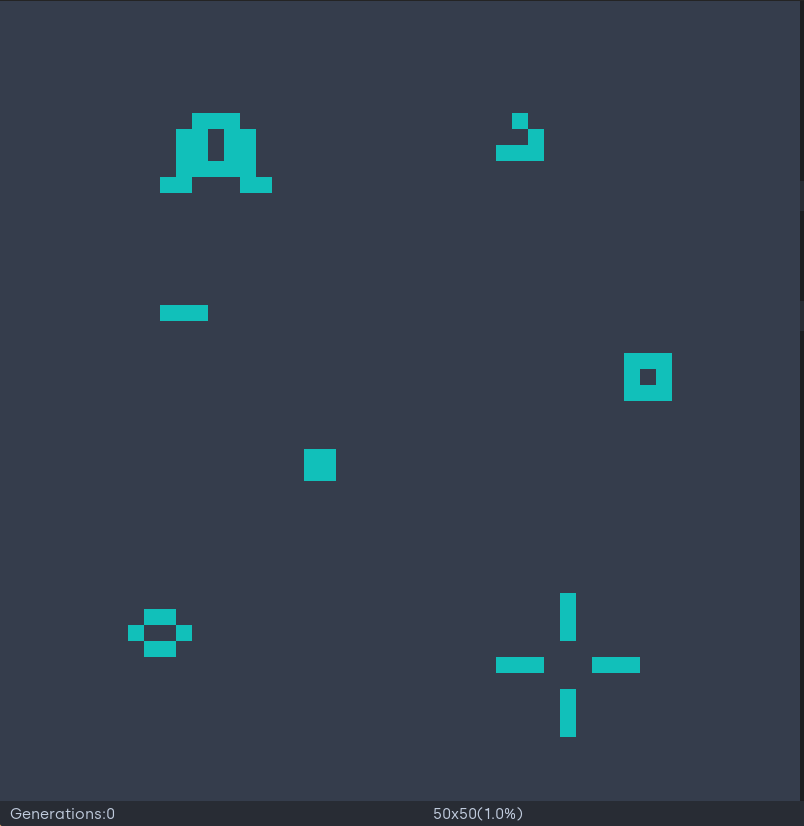
\includegraphics[width=8cm]{Imagenes/Configuracion_personalizada.png}
				\caption{Ejemplo de una configuración personalizada en un espacio de 50x50 con algunas de las estructuras comunmente encontradas en espacios de evolución suficientemente grandes o mediante trabajos de investigación especializados}
				\label{Configuracion_personalizada}
			\end{figure}
		
		\subsubsection{Limpiar, Guardar o Cargar espacio de evolución}
			Controlado por la triada de botones en la parte inferior derecha(Figura \ref{Space_configuration_buttons}), permite a la simulación limpiar completamente el espacio de evolución cambiando el estado de todas las células a 'Muertas' en ambos espacios(gráfico y lógico) y colocando en 0's el valor de las generaciones y células vivas.
			
			El par restante de botones son el complemento el uno del otro de una acción. La acción de guardar el espacio de evolución va a generar un nuevo archivo con extensión CSV guardándose en la carpeta \textit{saves}. Este archivo nuevo representa en 0's y 1's el estado del espacio de evolución actual, razón por la cual si se cuenta con un archivo con estas características se puede cargar de vuelta en una simulación.
			
			\hfill\break
			\hfill\break
			
			El proceso de cargado de un espacio guardado requiere que dentro de la carpeta \textit{saves} se tenga el archivo con la configuración deseada renombrado a \textit{upload.csv}, siendo imposible por el momento la elección específica de otro archivo e incluso generando un error si se acciona el botón de \textit{Upload} sin existir este archivo en la carpeta. Este proceso permite cargar configuraciones de espacios de evolución iguales o más pequeños que el espacio actual, centrándose la configuración cargada con respecto a filas y columnas si esta es más pequeña(Figura \ref{Centrado_configuracion_cargada}).
			
			\begin{figure}[!h]
				\centering
				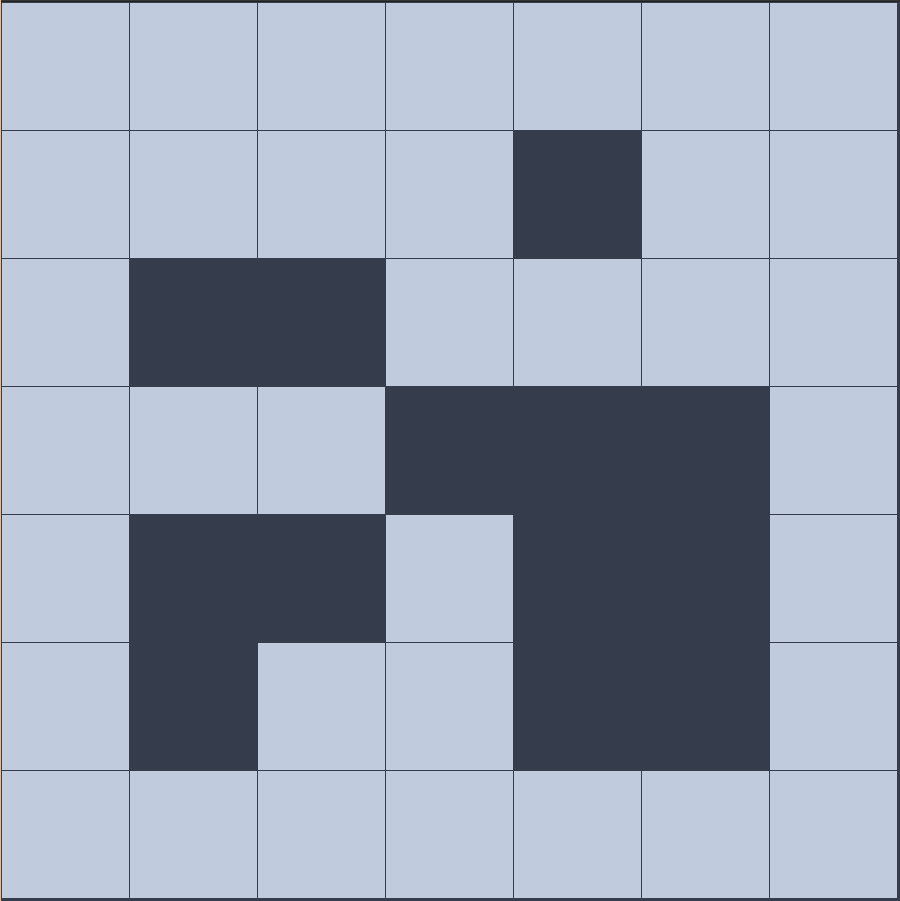
\includegraphics[width=7cm]{Imagenes/Ejemplo_configuracion_cargada.png}
				\caption{Ejemplo del centrado de una configuración de tamaño 5x5 cargada en un espacio de evolución 7x7}
				\label{Centrado_configuracion_cargada}
			\end{figure}
		
		\subsubsection{Cambio de colores}
			La simulación permite cambiar los colores de las células gráficas de ambos estados, contando para esto de un par de componentes gráficos(Figura \ref{Colores_celulas}) a los cuales al dar un click sobre estos cambiará su color, tanto el recuadro del input como el grid de las células gráficas que actualmente tengan el estado modificado, por el siguiente en la lista llamada \textit{COLORS\_LIST} en el módulo \textit{Constant}. Esta lista no es más que un conjunto de 13 tuplas con 3 elementos cada una, representando cada tupla un color en formato RGB.
			
			Por el momento el cambio de colores solo se logra de esta forma por lo que no es posible asignar un color específico no identificado en el módulo, sin embargo esta cantidad de colores generan una buena cantidad de combinaciones suficientes para un programa simulador de este tipo.

			Ejemplos del cambio de colores se notan en las figuras: \ref{Configuracion_personalizada}, \ref{Evolucion_100x100}, \ref{Evolucion_300x300}, \ref{Evolucion_500x500} y \ref{Evolucion_1000x1000}		
		
		\newpage
		\subsubsection{Proceso de evolución}
			La función para el cálculo de la siguiente generación se encuentra en los módulos \textit{CellularAutomaton} y \textit{CUDACellularAutomaton} de las sección \textit{Código Fuente}.
			
			El proceso del cálculo de una nueva generación consiste en el cálculo del estado de todas las células que conforman al espacio a través de la contabilización del número de células vecinas en la vecindad de Moore de la célula ancla(Célula central en la ventana llamada vecindad de Moore con tamaño 3x3).
			
			Esta función es sin duda el algoritmo más relevante en toda la simulación, y que requiere de un par de recursos para ser calculada:
			\begin{itemize}
				\item Espacio toroidal: Este recurso describe el comportamiento del espacio de evolución durante el cálculo de una nueva generación, en el que al igual que un toroide(volúmen geométrico con forma de dona) se enlazan los extremos de las filas y columnas del espacio. Este recurso se utiliza para asegurar la existencia de la vecindad de Moore en cada una de las células, siendo especificamente beneficiadas todas las células que existen en las filas y columnas extremos del espacio. \\ Existen algunas alternativas para lograr este comportamiento, más la solución utilizada en este trabajo fue la adición de un \textit{padding}(Filas y columnas extras en los extremos de un \textit{array}) en el que se replican los valores de los extremos contrarios, resultando en una amplicación del \textit{array} del espacio de evolución en 2 filas y 2 columnas en las primeras 2 dimensiones.
				\item Regla de evolución: Definida en una tupla cuadruple de valores enteros, las reglas de evolución dictan las condiciones en las que el estado de una célula cambia(Permanece viva, Muere o Nace).\\ El primer par de valores funciona como un rango del número de células vecinas vivas para que la célula ancla permanezca viva, mientras el último par es el rango de células vecinas vivas bajo las que una célula ancla Muerta cambie su estado a Viva(Nacimiento).
			\end{itemize}
		
		Este proceso se lleva a cabo en una función que itera sobre todos los elementos del espacio de evolución()con excepción de los elementos en la última fila y última columna), esto se debe a que la conformación de las vecindades de Moore se realizan tomando como célula ancla la célula ubicada 1 columna y 1 fila siguiente del elemento que realmente localiza la tupla de las variables iteradoras \textit{x,y}. A partir de que se conforma una ventana de 3x3, se algoritmo básico explicado al principio de la sección, se contabiliza el número de vecinos, se aplica la regla de evolución en función del estado actual de la célula ancla y el número de vecinos vivos, y finalmente el estado de la nueva célula se guarda en la misma ubicación bidimensional pero en el segundo elemento del \textit{array} tridimensional, conservando el estado anterior del espacio de evolución en el primer elemento de la tercer dimensión en el \textit{array}. Cuando se obtiene el nuevo valor de la célula, se actualiza inmediatamente el estado y color de la célula gráfica en la interfaz, conservando la congruencia entre los espacios lógicos y gráficos. Finalmente cuando se han calculado todos los nuevos estados de las células en la nueva generación, se trasladan los nuevos valores de la nueva generación al primer elemento de la 3° dimensión del \textit{array}(pasan a formar parte de los valores de la generación actual), y se retornan a 0 los valores del segundo elemento en la 3° dimensión.
		
		Este proceso es ligeramente diferente cuando se utiliza una mejora del rendimiento con GPU, pues el array que se copia desde el dispositivo al \textit{host} no es como tal el espacio de evolución, sino un \textit{array} que indica en que posiciones las células gráficas deben cambiar su estado actual unicamente, pues como ya se ha mencionado anteriormente los \textit{array} de espacio de evolución actualizados permanecen en la memoria de la GPU.
		
		\begin{landscape}
			
			\hfill \break
			\hfill \break
			\hfill \break
			\hfill \break
			\hfill \break
			\hfill \break
			\hfill \break
			\begin{table}[!h]
				\centering
				\begin{tabular}{c c}
					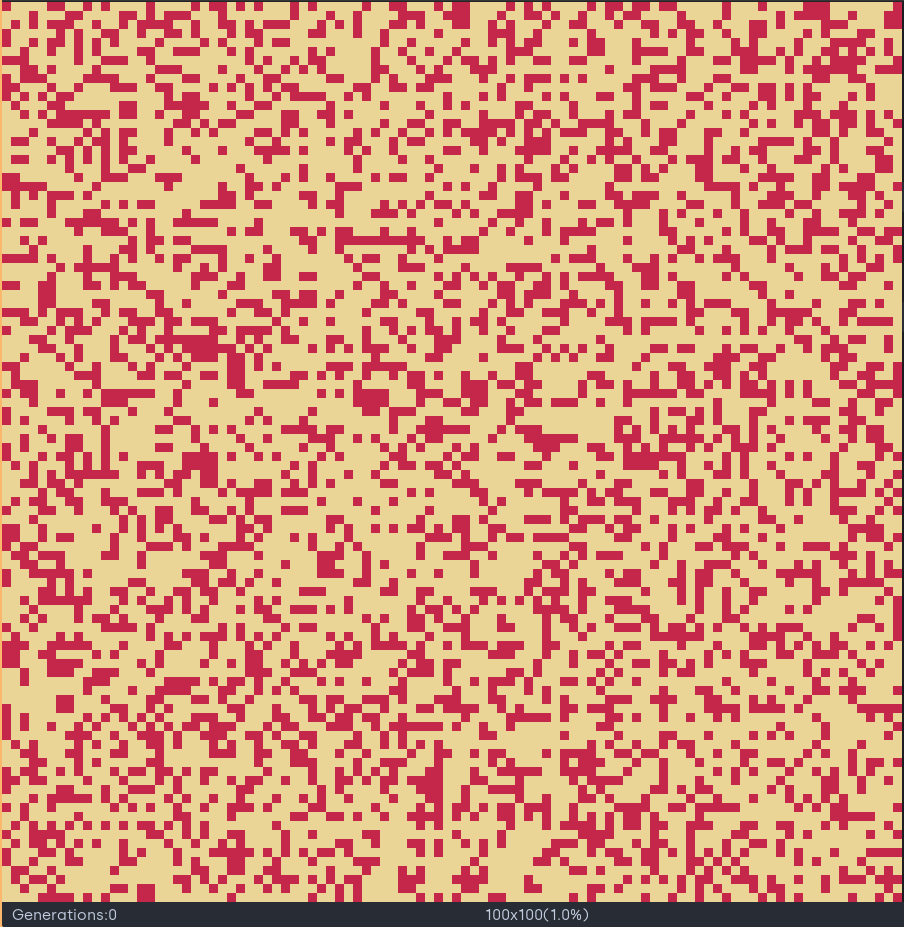
\includegraphics[width=11cm]{Imagenes/Evolucion_100x100_0Gen.png} &
					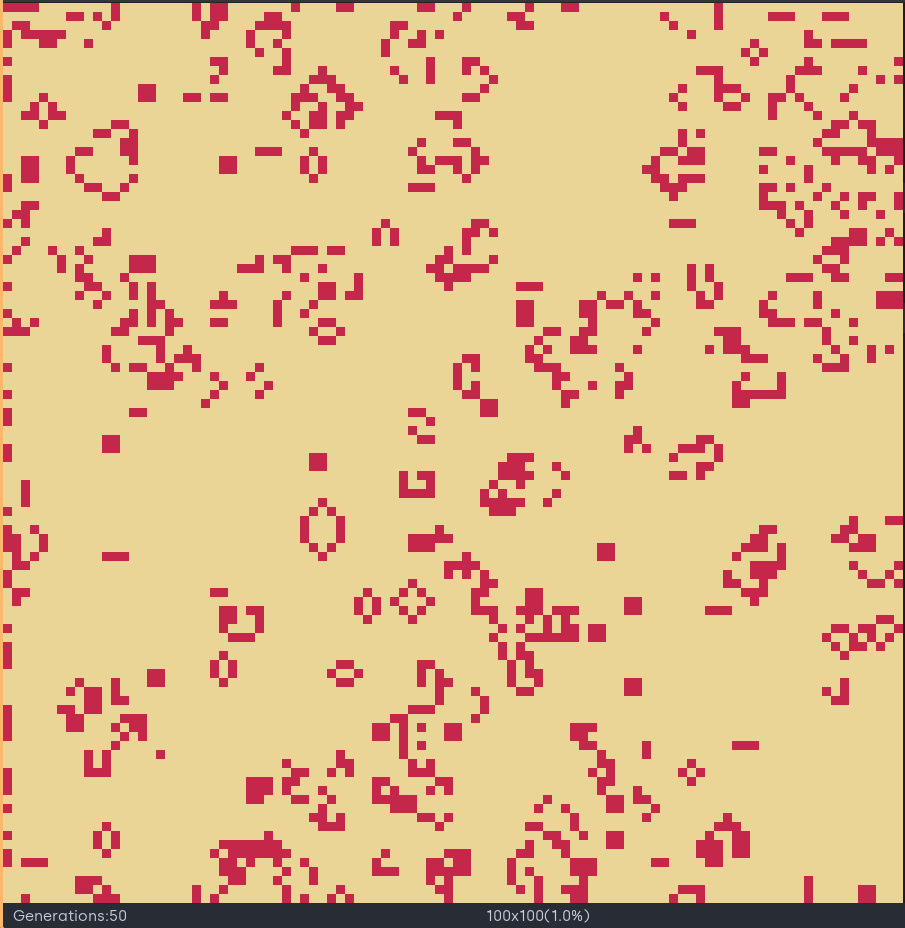
\includegraphics[width=11cm]{Imagenes/Evolucion_100x100_50Gen.png}
				\end{tabular}
				\caption{Ejemplo de la evolución de un espacio de tamaño 100x100 después de 50 Generaciones al partir de una configuración inicial con 45\% de probabilidad para el estado 0 \\ Colores: Amarillo $\rightarrow$ Muertas, Rojo $\rightarrow$ Vivas}
				\label{Evolucion_100x100}
			\end{table}
			
			\newpage
			\hfill \break
			\hfill \break
			\hfill \break
			\hfill \break
			\hfill \break
			\hfill \break
			\hfill \break
			\begin{table}[!h]
				\centering
				\begin{tabular}{c c}
					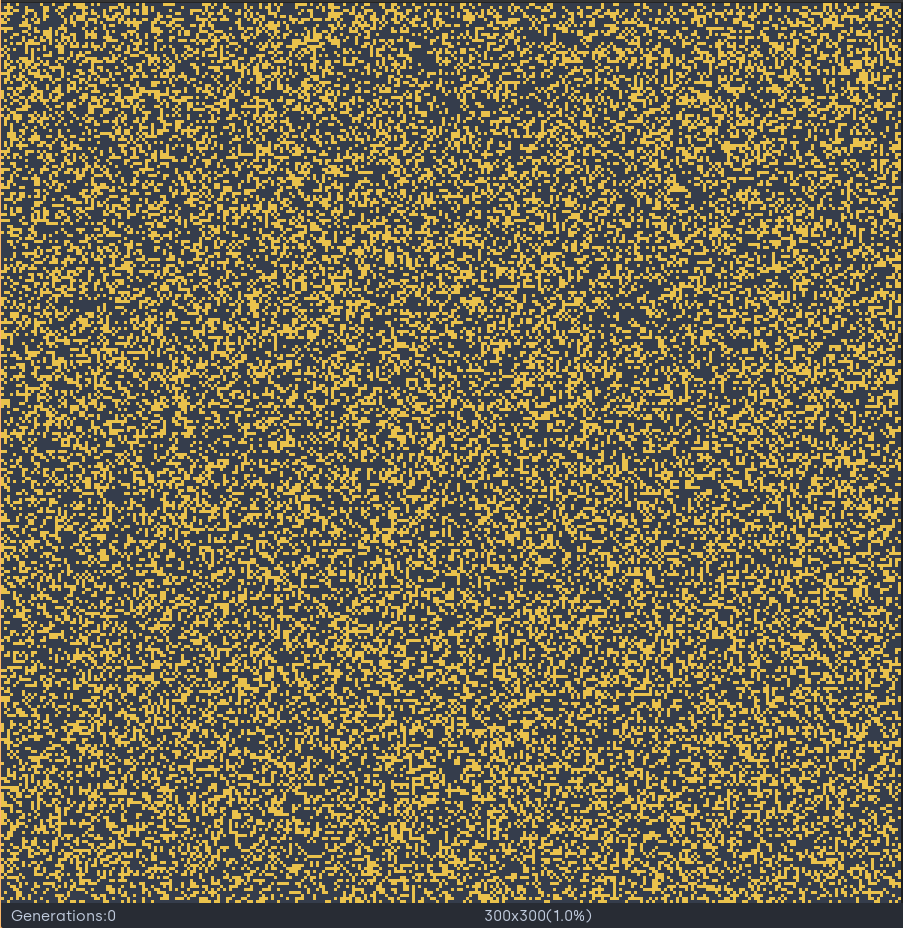
\includegraphics[width=11cm]{Imagenes/Evolucion_300x300_0Gen.png} &
					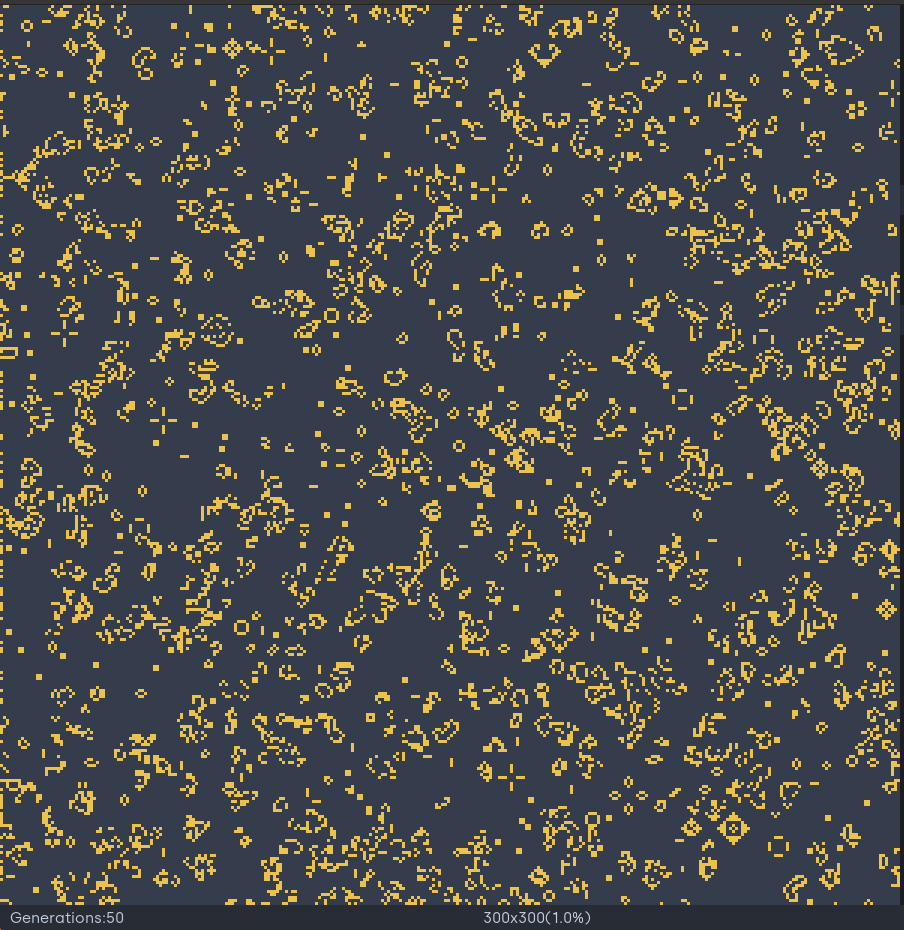
\includegraphics[width=11cm]{Imagenes/Evolucion_300x300_50Gen.png}
				\end{tabular}
				\caption{Ejemplo de la evolución de un espacio de tamaño 300x300 después de 50 Generaciones al partir de una configuración inicial con 45\% de probabilidad para el estado 0 \\ Colores: Negro $\rightarrow$ Muertas, Amarillo $\rightarrow$ Vivas}
				\label{Evolucion_300x300}
			\end{table}
		
			\newpage
			\hfill \break
			\hfill \break
			\hfill \break
			\hfill \break
			\hfill \break
			\hfill \break
			\hfill \break
			\begin{table}[!h]
				\centering
				\begin{tabular}{c c}
					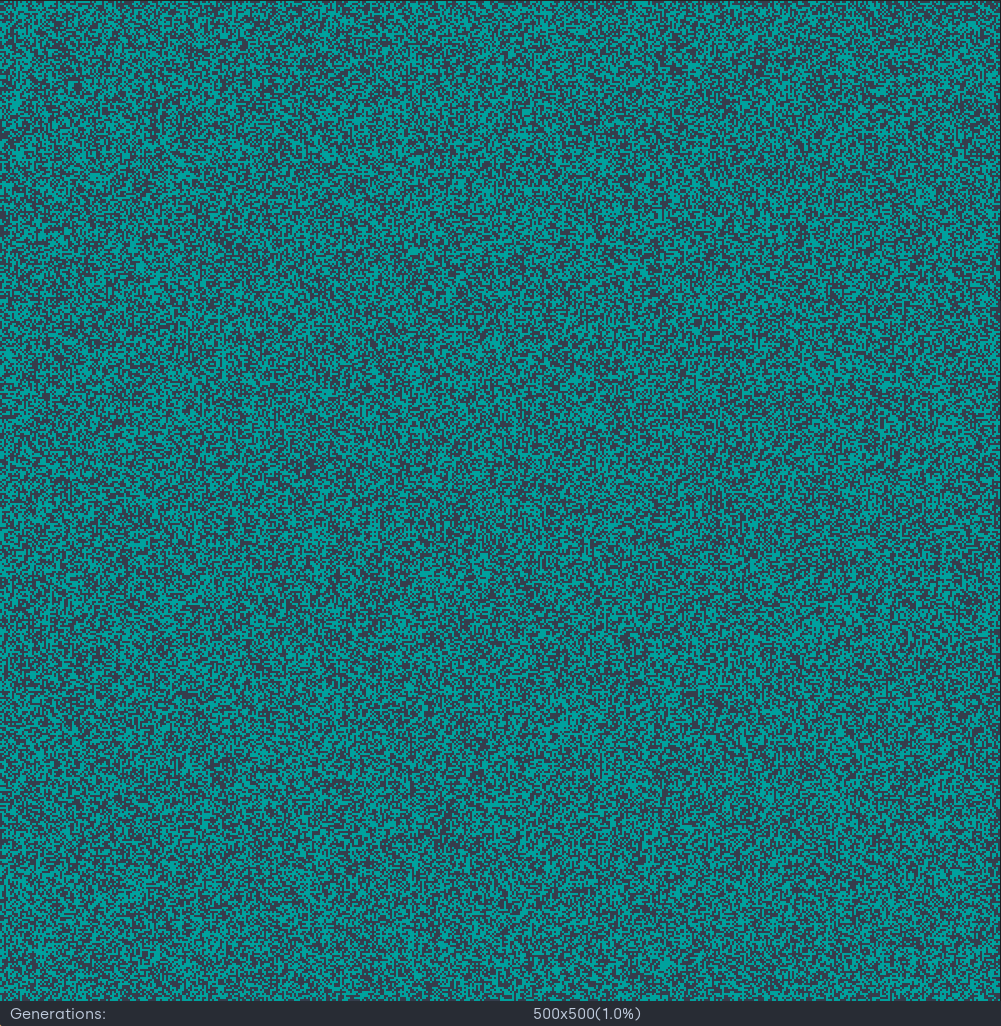
\includegraphics[width=11cm]{Imagenes/Evolucion_500x500_0Gen.png} &
					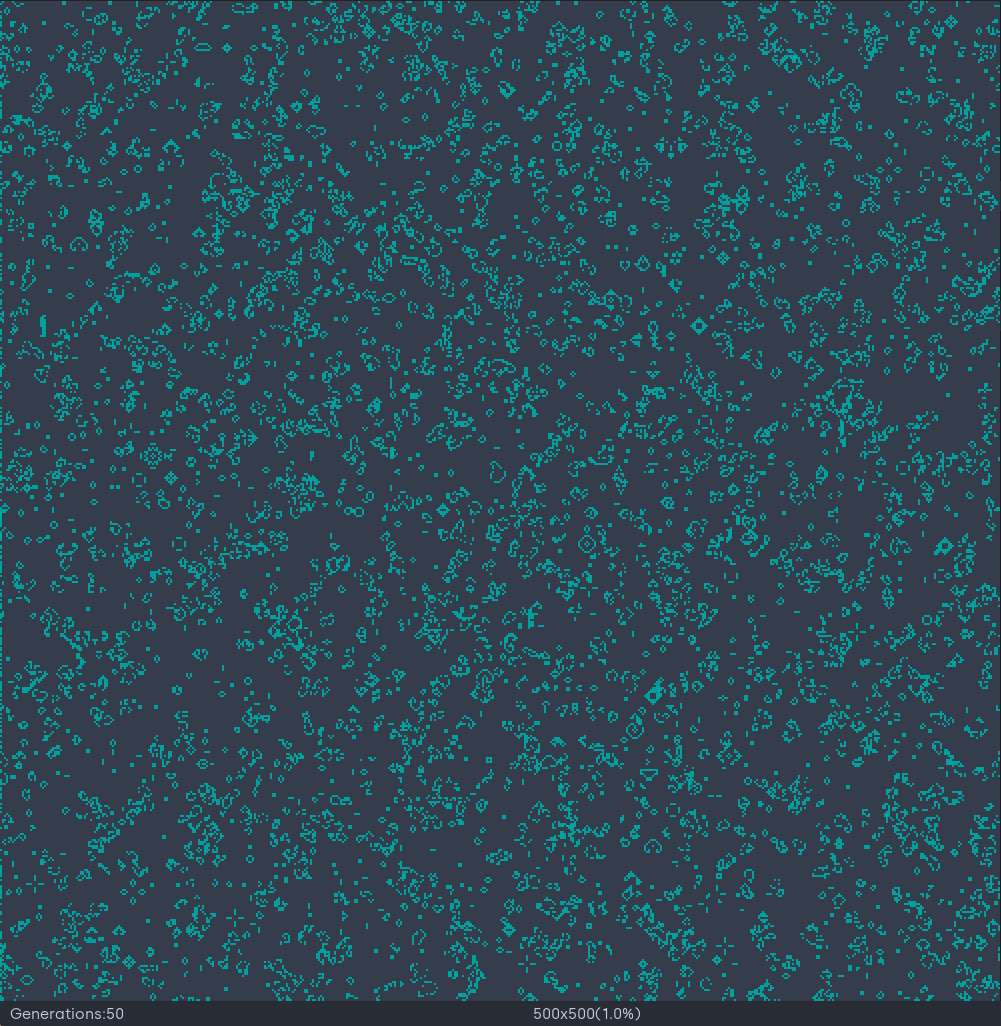
\includegraphics[width=11cm]{Imagenes/Evolucion_500x500_50Gen.png}
				\end{tabular}
				\caption{Ejemplo de la evolución de un espacio de tamaño 500x500 después de 50 Generaciones al partir de una configuración inicial con 45\% de probabilidad para el estado 0 \\ Colores: Negro $\rightarrow$ Muertas, Azul $\rightarrow$ Vivas}
				\label{Evolucion_500x500}
			\end{table}
		
			\newpage
			\hfill \break
			\hfill \break
			\hfill \break
			\hfill \break
			\hfill \break
			\hfill \break
			\hfill \break
			\begin{table}[!h]
			\centering
			\begin{tabular}{c c}
				
\includegraphics[width=11cm]{Imagenes/Evolucion_1000x1000_0Gen.png} &
				
\includegraphics[width=11cm]{Imagenes/Evolucion_1000x1000_50Gen.png}
			\end{tabular}
			\caption{Ejemplo de la evolución de un espacio de tamaño 1000x1000 después de 50 Generaciones al partir de una configuración inicial con 45\% de probabilidad para el estado 0 \\ Colores: Negro $\rightarrow$ Muertas, Blanco $\rightarrow$ Vivas}
			\label{Evolucion_1000x1000}
			\end{table}
		\end{landscape}
	
	\subsection{Graficación}
		Parte de un análisis estadístico de los espacios de evolución, se tiene la graficación de parámetros que ayuden a describir de alguna u otra forma al espacio de evolución, y en más específico la generación actual.
		
		Se habilita en la simulación la graficación de 3 parámetros mediante el uso de 3 botones en su respectiva sección(Figura \ref{Botones_graficacion})
		
		\subsubsection{Densidad}
			Primer botón del arreglo de 3. Este butón graficará cuando presionado, el número de células vivas(densidad) de todas las generaciones evolucionadas hasta el momento.
			
			Su implementación es bastante sencilla, requiriendo únicamente de una lista a la que se le agregan el número de células nuevas después de calcular una nueva evolución.
			
			\begin{table}[!h]
				\centering
				\begin{tabular}{c c}
					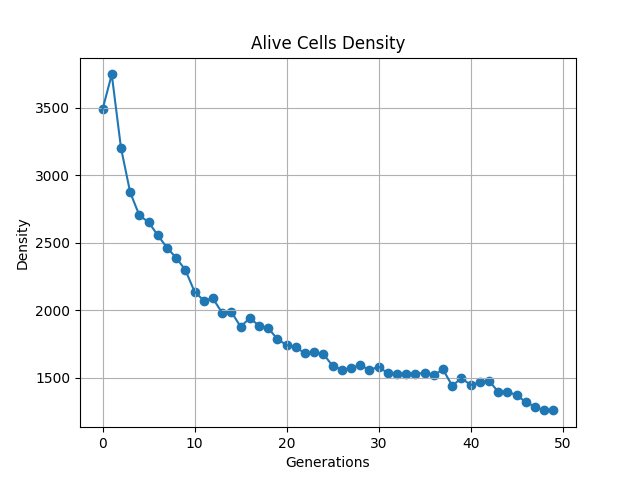
\includegraphics[width=9cm]{Imagenes/Densidad_100x100_50Gen.png} & 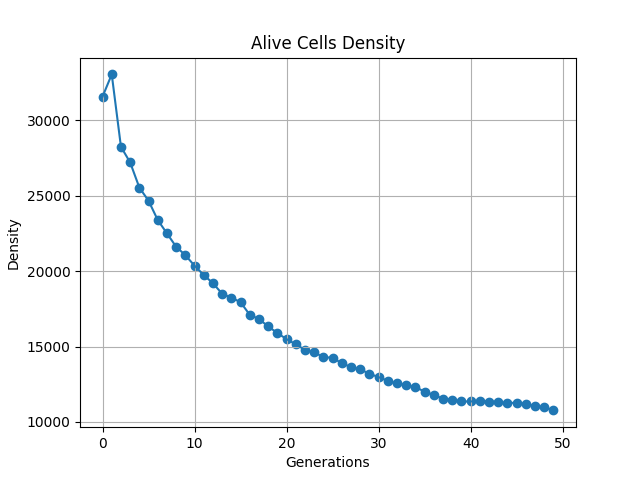
\includegraphics[width=9cm]{Imagenes/Densidad_300x300_50Gen.png} \\
					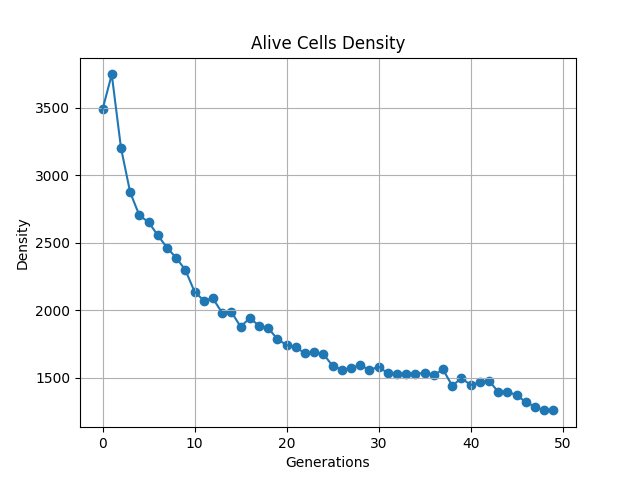
\includegraphics[width=9cm]{Imagenes/Densidad_100x100_50Gen.png} & 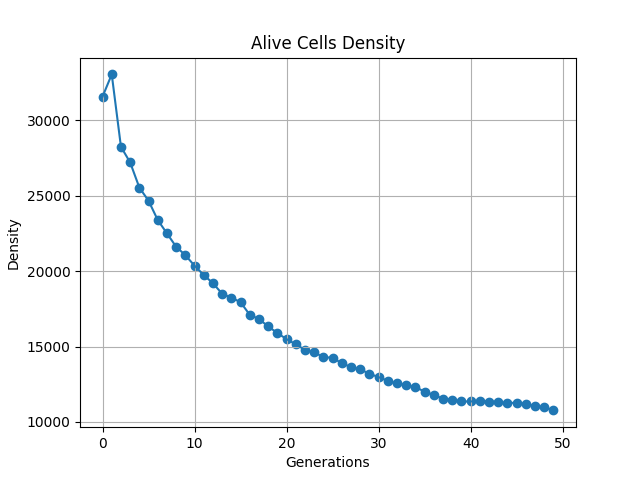
\includegraphics[width=9cm]{Imagenes/Densidad_300x300_50Gen.png} 
				\end{tabular}
				\caption{Gráficas de densidad después de 50 generaciones para diferentes tamaños de espacios de evolución iniciadas con configuraciones aleatorias con 45\% de probabilidad para el estado 1\\ Tamaños de los espacios de evolución, de izquierda a derecha y arriba hacia abajo: a) 100x100, b) 300x300, c) 500x500, d) 1000x1000}
			\end{table}
		
		\newpage
		\subsubsection{Logaritmo Densidad}
			Mismo funcionamiento e incluso parámetro que la gráfica de densidad, con la única particularidad de graficarse el logaritmo de esta: $log_{10}(Densidad)$
			
			\begin{table}[!h]
				\centering
				\begin{tabular}{c c}
					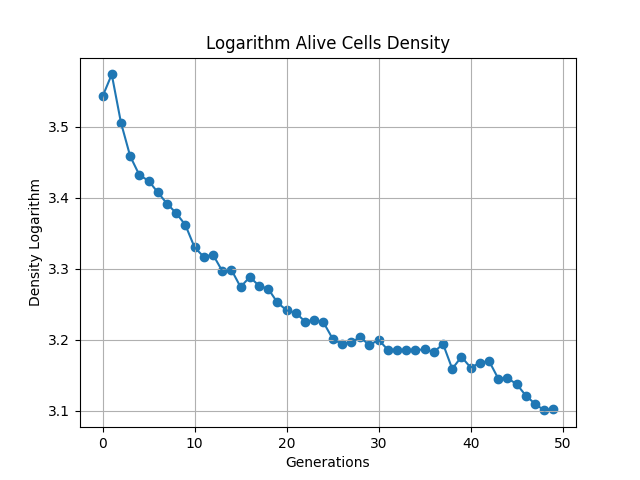
\includegraphics[width=9cm]{Imagenes/Densidad_logaritmo_100x100_50Gen.png} & 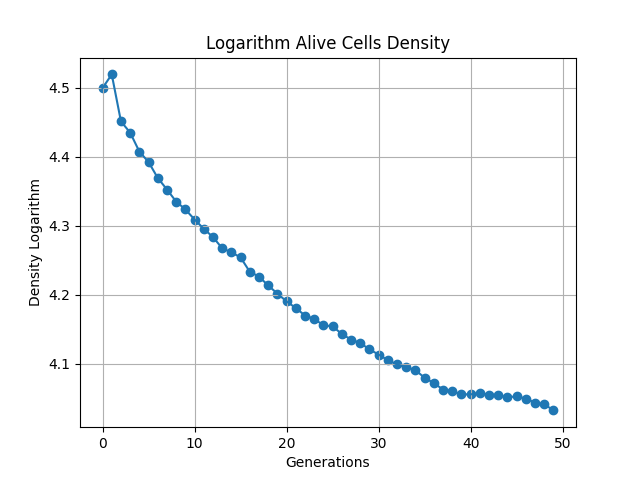
\includegraphics[width=9cm]{Imagenes/Densidad_logaritmo_300x300_50Gen.png} \\
					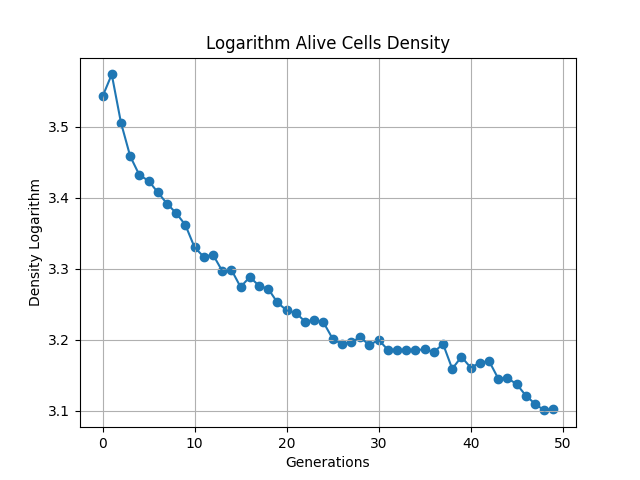
\includegraphics[width=9cm]{Imagenes/Densidad_logaritmo_100x100_50Gen.png} & 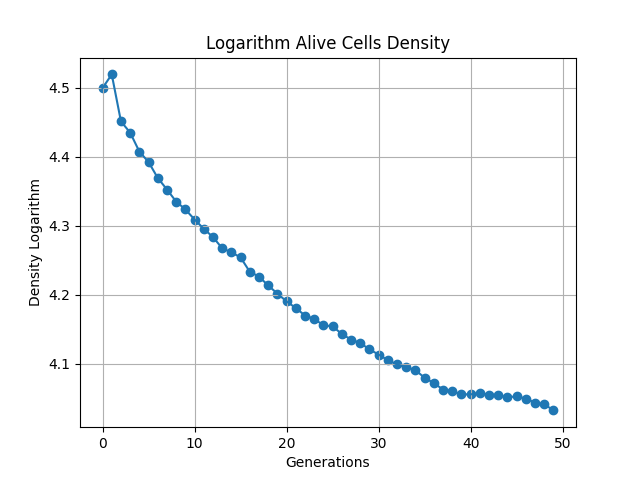
\includegraphics[width=9cm]{Imagenes/Densidad_logaritmo_300x300_50Gen.png} 
				\end{tabular}
				\caption{Gráficas del logaritmo de la densidad después de 50 generaciones para diferentes tamaños de espacios de evolución iniciadas con configuraciones aleatorias con 45\% de probabilidad para el estado 1\\ Tamaños de los espacios de evolución, de izquierda a derecha y arriba hacia abajo: a) 100x100, b) 300x300, c) 500x500, d) 1000x1000}
			\end{table}
		
		\newpage
		\subsubsection{Entropia}
			La entropía de Shannon en el ámbito de la información se trata de una cantidad que indica le incertidumbre de una fuente de información, también pudiendo interpretarse como la cantidad de información promedio que contienen los símbolos utilizados. Los símbolos con menor probabilidad de aparición serán los que aporten mayor información a la medida, de forma que llegan aumentar o disminuir el valor de esta.
			
			Cuando se tenga una distribución homogenea de los símbolos existentes(cada símbolo diferente tendrá la misma probabilidad), entonces la entropía toma el valor de 1, mientras más símbolos diferentes en distribución heterogea existan en un conjunto, más alejado el valor de la entropía se encontrará del 1.
			
			Partiendo del predicado "La entropía mide la cantidad de certidumbre en la incertidumbre", resulta natural asocial la certidumbre de algo que pase con la probabilidad \textit{P}, entonces la incertidumbre debe ser el inverso de la Probabilidad $\frac{1}{P}$. La multiplicación de los dos términos satisface el predicado, sin embargo si se implementara de esta forma, obtendríamos que cuando un símbolo tiene probabilidad 1 la medida de incertidumbre sería igualmente 1, pero lo correcto sería que este fuera 0 pues estamos completamente seguros que cualquier símbolo escogido siempre será el mismo, por esta razón se implementa el logaritmo:
			
			$$
				H = \sum p(x) log\left(\frac{1}{p(x)}\right)
			$$
			
			Aplicando propiedades de logaritmos:
			$$
				H = \sum p(x)( log(1) - log(p(x)) ) = \sum(p(x)(0) - p(x)log(p(x)))
			$$
			Resultando finalmente en la ecuación planteada por Claude Shannon en 1948:
			$$
				H = -\sum p(x) log(p(x))
			$$
			
			A partir de esta ecuación lo que se quiere implementar para su graficación en la simulación, es calcular el desorden o deferencias, en las vecindades existentes en un espacio de evolución después de calcular su nueva generación. Para esto primero se requiere contabilizar la frecuencia de aparación de cada tipo de vecindad en el espacio, la solución utilizada para esta contabilización fue la de asignar un número único a cada tipo de vecindad, y la forma más sencilla es tomando a los elementos de la vecindad como un número binario, donde naturalmente la posición de cada elemento está ponderado y le corresponde una potencia de 2 para su conversión a decimal. Al convertir esta matriz con sus valores a un valor decimal, este valor sirve como id que identifica al tipo de vecindad permitiendo el incremento de su frecuencia cuando contabilizado.
			
			Después de la contabilización de frecuencias de cada vecindad se realiza la división por el número de elementos en el espacio, obteniendo así la probabilidad de aparición de cada vecindad en esa generación para el espacio de evolución.
			
			Finalmente tan solo resta aplicar la ecuación de la Entropía de Shannon y mediante un for calcular la entropía de esta vecindad, restándola al resultado general.
			
			Afortunadamente para el contexto de la optimización, el cálculo de la frecuencia de las vecindades en un espacio de evolución es un algoritmo paralelizable(sucede lo mismo para el cálculo final del entropía por cada vecindad, sin embargo este proceso se realiza en CPU pues requiriría el transporte de un \textit{array} con 512 elemento de la memoria \textit{host} a la GPU cada vez que se calculara, resultando en tiempo de procesamiento muy iguales tan solo por esta acción), significando que es posible su cálculo con una función \textit{Kernel} en la GPU. Esta función y su algoritmo de ejecución es explicada a detalle en la Subsección \textbf{Aceleración por GPU}, limitándose en esta sección a indicar su uso cuando la variable de configuración aceleración por GPU se encuentra activa.
			
			Un ejemplo de los resultados obtenidos de la graficación de la Entropía para un espacio de evolución después de algunas generaciones se observa en la figura \ref{Entropia_graficas}
			
			\newpage
			\begin{table}[!h]
				\centering
				\begin{tabular}{c c}
					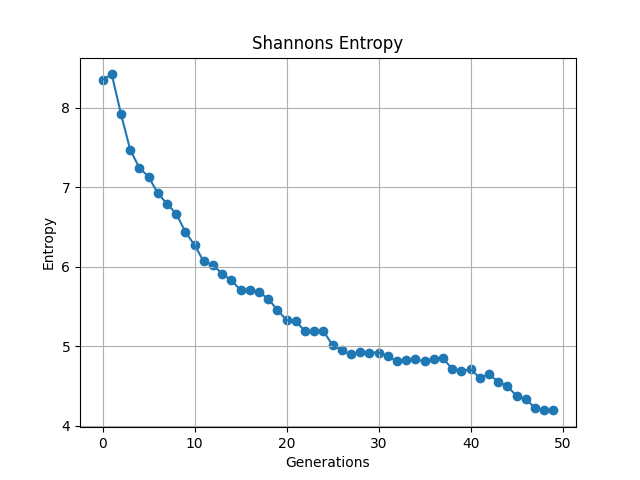
\includegraphics[width=9cm]{Imagenes/Entropia_100x100_50Gen.png} & 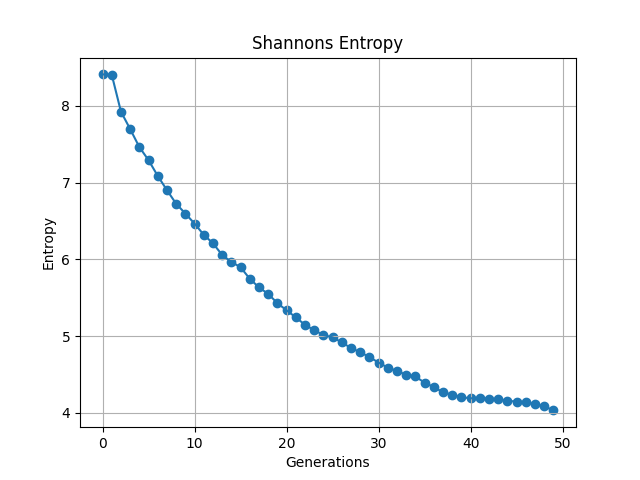
\includegraphics[width=9cm]{Imagenes/Entropia_300x300_50Gen.png} \\
					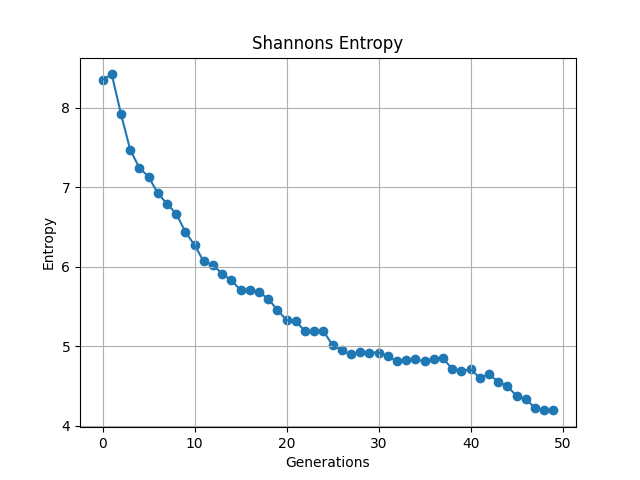
\includegraphics[width=9cm]{Imagenes/Entropia_100x100_50Gen.png} & 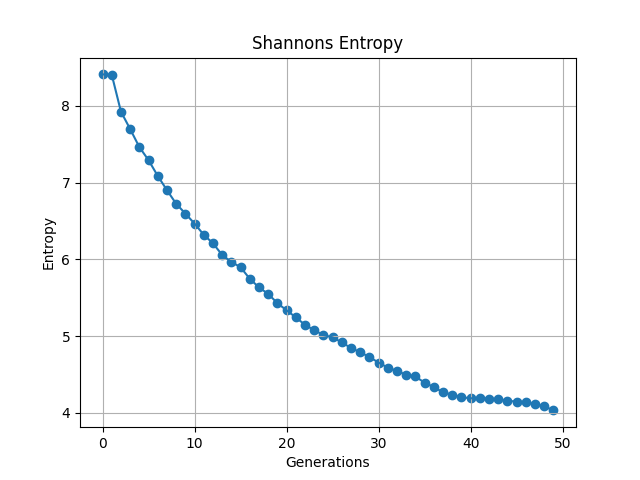
\includegraphics[width=9cm]{Imagenes/Entropia_300x300_50Gen.png} 
				\end{tabular}
				\caption{Gráficas de la entropía de Shannon para las vecindades después de 50 generaciones para diferentes tamaños de espacios de evolución iniciadas con configuraciones aleatorias con 45\% de probabilidad para el estado 1\\ Tamaños de los espacios de evolución, de izquierda a derecha y arriba hacia abajo: a) 100x100, b) 300x300, c) 500x500, d) 1000x1000}
				\label{Entropia_graficas}
			\end{table}
		
\newpage
\section{Conclusión}
	El objetivo del documento es el de mostrar el funcionamiento de la aplicación creada como simulador de evoluciones de espacios de autómatas en 2D. Inspirado principalmente en el concepto y funcionamiento del Juego de la Vida de Conway, se logró exitosamente implementar un formato de regla de tuplas de 4 valores, expandiendo el conjunto de posibles reglas y por lo tanto comportamientos de simulaciones.
	
	De los requisitos funcionales necesarios planteados para la creación del simulador, se lograron cumplir con todos ellos, siendo únicamente un requisito no funcional el que ha quedado pendiente de implementación y es el añadido de una función de Zoom. Este único requisito es algo complejo de implementar tomando en cuenta las pocas herramientas disponibles en PyGame para su desarrollo, implicando que su implementación y diseño sea completamente partiendo desde 0.
	
	Se resalta que del simulador, se trabajo en el desarrollo de los componentes gráficos aún con las pocas herramientas que ofrece la biblioteca PyGame, requiriendo en su gran parte su diseño desde 0. Todo esto se realizó tratando de cumplir el objetivo de implementar un simulador que no solo funcional, fuera intuitivo para utilizar y estéticamente agradable en su interfaz gráfica.
	
	Importante señalar que en un principio del desarrollo el aspecto de la optimización no presentaba gran dificultad por lo reducido de las dimensiones de los espacios con los que se trataba, así como los limitados componentes gráficos, aún cuando por sus diferentes funciones desencadenadas por eventos, los componentes como botones y el \textit{slider} requieren de un consumo de tiempo de ejecución en CPU para validación y ejecución de estos eventos. Sin embargo a medida que el simulador crecía en componentes y se iniciaban las pruebas con dimensiones mayores cumpliendo con los requisitos de espacios de 1000x1000, el desempeño se empezó a mostrar como detrimento mayor en la ejecución del simulador. 
	
	Una alternativa que resulto ser útil, al menos ahorrando ciclos de procesamiento en la ejecución de procesos pertenecientes a la lógica y otorgando resultados rápidos en tiempo de operaciones pesadas, grandes y tardadas sobre \textit{arrays}, fue la paralelización de procesos y el uso de la GPU para la optimización del simulador. Aún con esta gran carga liberada del CPU, en dimensiones grandes el simulador aún muestra un desempeño un poco reducido pero bastante aceptable, su razón fue identificada en el refresco frecuente de todos los elementos gráficos presentes en la interfaz, más sin embargo esta oportunidad de mayor optimización no pudo ser tratada en este simulador, al menos en la última versión existente en la fecha que se escribe el documento, pero ciertamente me permitió concientizarme de esta importante modificación, obligando que desde un principio el simulador siguiente de Autómatas Celulares Elementales en 1D, sean implementadas técnicas especializadas de optimización gráfica otorgando resultados importantes con posibilidades de manejo de grandes espacios de evolución con apenas diferencia en rendimiento de espacios más pequeños.
	
	Este simulador además de permitir comprender y explorar la búsqueda de la solución para la evolución de los autómatas celulares en 2D regidos por la regla de la vida, me brindó la oportunidad de estudiar soluciones de optimización mediante paralelización de funciones con los \textit{Kernels} de una tarjeta gráfica, permitiéndome conseguir el aprendizaje de una herramienta sumamente útil en otras ramas de la carrera que también forman parte de mi interés profesional, como sucede con el \textit{Machine Learning} donde la paralelización se utiliza para el entrenamiento de modelos y redes neuronales en el \textit{Deep Learning}, o también para operaciones sobre imágenes en la rama de Análisis de Imágenes y Visión por Computadora, etc. 

\newpage
\section{Código Fuente}
	El código fuente también puede ser encontrado en el repositorio de GitHub para su consulta o descarga para prueba: \textbf{https://github.com/LaloValle/Game-of-life}

	El código fuente está conformado por un total de 6 módulos de Python y un archivo principal donde se cuenta con la función main que controla el flujo principal del programa y contexto gráfico para la biblioteca PyGame.
	
	\subsection{Módulos}
		Los módulos son archivos de código Python que agrupan clases, funciones, constantes, etc. que semánticamente se encuentran correlacionadas bajo un contexto común. Los siguientes módulos contienen en su mayoría Clases que definen componentes lógicos, nodos de un sistema, componentes gráficos; también pueden contener Constantes de uso extendido entre los módulos del programa.
		
		\subsubsection{Constant}
			Módulo que integra algunos recursos constantes comúnes a varios de los módulos en la simulación. Los recursos incluyen tuplas de colores en formato RGB, instancias de fuentes para PyGame, matrices de conversión, y reglas predefinidas para el proceso de evolución.
			
			\lstinputlisting[language=Python]{../Constant.py}
			
		\subsubsection{Layouts}
			Parte de los módulos relacionados a los gráficos, este módulo está conformado por clases que como elementos utilizados en interfaces gráficas, funcionan como herramientas que dan estructura a los elementos o que aportan cierta funcionalidad relacionada con su estructuración. Estos elementos pueden tener, o no, una representación gráfica visual.
			
			\paragraph{Clase Grid}
				Mencionada en secciones anteriores, esta clase define un componente estructural sin representación visual, pero que provee métodos útiles para la estructuración automática de elementos en un formato tipo tabla.
				
			\paragraph{Clase SideBar}
				Elemento gráfico estructural con representación visual como de un gran rectángulo que abarca lo alto de la ventana, es utilizada para agrupar visualmente elementos gráficos, y proveer una posición de referencia para colocar otros componentes. En particual esta clase es una clase \textit{Singleton}, de forma que en el contexto de la simulación existe una instancia única, por lo que la definición y colocación de elementos como botones, etc. Se realiza directamente en la clase.
				
			\paragraph{Clase BottomBar}
				Elemento gráfico estructural con representación visual como un delgado rectángulo ubicado en la parte inferior de la ventana ocupando todo su ancho. Con comportamiento parecido a la clase SideBar, sirve como agrupador visual y como referencia para otros componentes, siendo en este caso el de los textos que indican las variables dinámicas de la simulación.
			
			
			\lstinputlisting[language=Python]{../Layouts.py}
			
		\subsubsection{GraphicalComponents}
			Módulo relacionado a los gráficos, integrando de hecho clases que definen componentes gráficos con representación visual.
			
			\paragraph{Control}
				Definida como una clase modelo o abstracta, define el formato o esqueleto básico de muchos de los componentes \textit{Sprite} en el mismo módulo.
				
			\paragraph{MousePointer}
				Única clase de componente gráfico sin representación visual en este módulo. Su principal objetivo es permitir identificar el colapso de otros componentes \textit{Sprite} dentro de la interfaz con el cursor.
				
				Consiste primordialmente en un \textit{Sprite} rectángulo de una tamaño generalmente pequeño como de 1px por 1px, que se mueve a la misma posición que sigue el cursor.
				
			\paragraph{CircularButton}
				Clase que representa un componente gráfico con visualización, tiene generalmente un forma redondeada de botón. Esta trata de imitar la estética y funcionalidad de un botón con funciones al desencadenarse un evento(hover, click, stop\_click, etc.)
				
			\paragraph{Text}
				Clase de componente gráfico que incluye texto en la interfaz gráfica. Esta clase provee métodos para el manejo sencillo del texto
				
			\paragraph{Slider}
				Clase de componentes gráfico compuesto con representación visual. El principal objetivo de esta clase es modelar la estética y funcionamiento normal de un \textit{Slider} encontrado en cualquier interfaz grafica, proveyendo métodos para el manejo de eventos, etc.
				
			\paragraph{Input}
				Clase de componentes gráfico compuesto con representación visual. El principal objetivo de esta clase es modelar la estética y funcionamiento normal de un \textit{Input} encontrado en cualquier interfaz grafica y más comunmente en formularios, proveyendo métodos para el manejo de eventos, etc.
				
			\paragraph{Section}
				Clase de componente gráfico con representación visual. Este componente funge únicamente como separadador visual de secciones, y aunque podría utilizarse como referencia para la colocación de elementos, su objetivo principal es visual y nadamás.
				
			
			\lstinputlisting[language=Python]{../GraphicalComponents.py}
		
		\subsubsection{Graphics}
			Módulo que integra en su definición la clase \textbf{GameGraphics}, la cuál bien podría tratarse como un nodo del sistema, encargándose en específico de la coordinación gráfica entre elementos gráficos, eventos y comunicación con el nodo lógico principal de la simulación. Su comportamiento definido por los métodos y atributos que maneja podría definirla como una clase \textit{Front-End} del programa de simulación.
			
			Así mismo conjunta una segunda clase llamada \textbf{Cell}, siendo la definición de una célula gráphica. Esta clase hereda de la clase de PyGame \textit{Sprite}, permitiendole verificar colisiones con otros \textit{Sprites}, sin embargo no solo es una definición de esta clase gráphica, pues se añaden algunos métodos más que le permiten modificar su comportamiento y valores, exponiendo sus métodos como principal interfaz para la interacción con instancias de esta clase.
			
			\lstinputlisting[language=Python]{../Graphics.py}
			
		\subsubsection{CellularAutomaton}
			Módulo se integra únicamente de la clase \textbf{CellularAutomaton}, clase que por definición de las responsabilidades, métodos y atributos que maneja, puede ser considerado uno de los Nodos principales de la simulación. Esta clase se encarga del manejo de la lógica detrás de la simulación, definiéndose en esta métodos encargados de la configuración, evolución y comunicación externa para los espacios de evolución. Evidentemente y al igual que sucede con la clase \textbf{GameGraphics}, tiene una relación directa de comunicación con el nodo principal gráfico para mantener la consistencia de los espacios de células lógicos y gráficos.
			
			Los métodos de esta clase principalmente se enfocan en la creación, configuración, reinicio y evolución del espacio de autómatas, integrando a su vez métodos auxiliares que se exponen como interfaces de comunización con el nodo gráfico de la simulación.
			Se cuenta también con métodos encargados de la graficación de las diferentes mediadas estadísticas de los espacios, y el guardado y alzado de espacios desde archivos CSV.
			
			\lstinputlisting[language=Python]{../CellularAutomaton.py}
			
		\subsubsection{CUDACellularAutomaton}
			Módulo final de la simulación. Creado a partir del rendimiento limitado que se conseguia cuando se trabajaban con espacios de evolución de gran tamaño, buscando liberar carga de procesamiento del CPU y acelerar el tiempo de ejecución de algoritmos pesados en procesamiento y tiempo de ejecución.
			
			El módulo esta conformado por las funciones \textit{Kernel} y una clase que controla su ejecución.
			
			\paragraph{Kernel and CUDA Functions}
				Se ha desarrollado más extensamente cada una de las funciones definidas y su funcionamiento específico en la sección \textbf{Aceleración por GPU}, más no se encuentra de más recordar que estas funciones son implementaciones paralelizadas de procesos generalmente ejecutadas de forma secuencial en la CPU cuando se manejan estructuras de varios elementos como los \textit{array}. Utilizando la tecnología CUDA de Nvidia, se permiten crear un número de bloques con un número de hilos por cada bloque, siendo habitual la definición de tantos hilos como elementos en el \textit{array}, implicando que el código de la función sea tomando en cuenta la operación con 1 elemento de ese array pero por la paralelización la GPU estará trabajando el mismo código en cada uno de los elementos del \textit{array} en un teórico ciclo de reloj para el procesamiento secuencial del CPU.
			
			\paragraph{CUDACellularAutomaton}
				Clase principalmente usada como interfaz de comunicación entre el nodo lógico(\textbf{CellularAutomaton}) y las funciones aceleradas por hardware. También permite la coordinación y ejecución de funciones paralelizadas específicas según el estado y acciones solicitadas por el usuario en la simulación.
			
			\lstinputlisting[language=Python]{../CUDACellularAutomaton.py}
			
	\subsection{main.py}
		Archivo Python principal de la simulación, en este se maneja el cíclo principal de la aplicación gráfica, la instanciación de todos los elementos y nodos que manejan la simulación, variables y constantes de configuración general del programa.
		
		\lstinputlisting[language=Python]{../main.py}

\end{document}          